% $Header: /Users/joseph/Documents/LaTeX/beamer/solutions/generic-talks/generic-ornate-15min-45min.de.tex,v 90e850259b8b 2007/01/28 20:48:30 tantau $

\documentclass{beamer}

% Diese Datei enth�lt eine L�sungsvorlage f�r:


% - Vortr�ge �ber ein beliebiges Thema.
% - Vortragsl�nge zwischen 15 und 45 Minuten. 
% - Aussehen des Vortrags ist verschn�rkelt/dekorativ.



% Copyright 2004 by Till Tantau <tantau@users.sourceforge.net>.
%
% In principle, this file can be redistributed and/or modified under
% the terms of the GNU Public License, version 2.
%
% However, this file is supposed to be a template to be modified
% for your own needs. For this reason, if you use this file as a
% template and not specifically distribute it as part of a another
% package/program, I grant the extra permission to freely copy and
% modify this file as you see fit and even to delete this copyright
% notice. 




\mode<presentation>
{
  \usetheme{Warsaw}
  % oder ...
  
  \setbeamercovered{transparent}
  % oder auch nicht
}


\usepackage[german]{babel}
% oder was auch immer

\usepackage[latin1]{inputenc}
% oder was auch immer

\usepackage{times}
\usepackage[T1]{fontenc}
% Oder was auch immer. Zu beachten ist, das Font und Encoding passen
% m�ssen. Falls T1 nicht funktioniert, kann man versuchen, die Zeile
% mit fontenc zu l�schen.

\usepackage[bold,full]{complexity}
% for complexity symbols

\title{Diagonalisierung und polynomielle Hierarchie}


\author[Corvin Paul, Matthias Schimek] % (optional, nur bei vielen Autoren)
{Corvin Paul \and Matthias Schimek}
% - Der \inst{?} Befehl sollte nur verwendet werden, wenn die Autoren
%   unterschiedlichen Instituten angeh�ren.

\date
{13.05.2015}


\subject{Informatik}
% Dies wird lediglich in den PDF Informationskatalog einf�gt. Kann gut
% weggelassen werden.


% Falls eine Logodatei namens "university-logo-filename.xxx" vorhanden
% ist, wobei xxx ein von latex bzw. pdflatex lesbares Graphikformat
% ist, so kann man wie folgt ein Logo einf�gen:

% \pgfdeclareimage[height=0.5cm]{university-logo}{university-logo-filename}
% \logo{\pgfuseimage{university-logo}}



% Folgendes sollte gel�scht werden, wenn man nicht am Anfang jedes
% Unterabschnitts die Gliederung nochmal sehen m�chte.
\AtBeginSubsection[]
{
  \begin{frame}<beamer>{Gliederung}
    \tableofcontents[currentsection,currentsubsection]
  \end{frame}
}


% Falls Aufz�hlungen immer schrittweise gezeigt werden sollen, kann
% folgendes Kommando benutzt werden:

%\beamerdefaultoverlayspecification{<+->}



\begin{document}

\begin{frame}
  \titlepage
\end{frame}

\begin{frame}{Gliederung}
  \tableofcontents
  % Die Option [pausesections] k�nnte n�tzlich sein.
\end{frame}



% Da dies ein Vorlage f�r beliebige Vortr�ge ist, lassen sich kaum
% allgemeine Regeln zur Strukturierung angeben. Da die Vorlage f�r
% einen Vortrag zwischen 15 und 45 Minuten gedacht ist, f�hrt man aber
% mit folgenden Regeln oft gut.  

% - Es sollte genau zwei oder drei Abschnitte geben (neben der
%   Zusammenfassung). 
% - *H�chstens* drei Unterabschnitte pro Abschnitt.
% - Pro Rahmen sollte man zwischen 30s und 2min reden. Es sollte also
%   15 bis 30 Rahmen geben.



\section{Einleitung}

\subsection[Kurzversion des ersten Unterabschnittstitels]
{Erster Unterabschnittstitel}

\begin{frame}{�berschriften m�ssen informativ sein.\\
    Korrekte Gro�-/Kleinschreibung beachten.}{Untertitel sind optional.}
  % - Eine �berschrift fasst einen Rahmen verst�ndlich zusammen. Man
  %   muss sie verstehen k�nnen, selbst wenn man nicht den Rest des
  %   Rahmens versteht.

  \begin{itemize}
  \item
    Viel \texttt{itemize} benutzen.
  \item
    Sehr kurze S�tze oder Satzglieder verwenden.
  \end{itemize}
\end{frame}

\begin{frame}{�berschriften m�ssen informativ sein.}

  Man kann Overlays erzeugen\dots
  \begin{itemize}
  \item mit dem \texttt{pause}-Befehl:
    \begin{itemize}
    \item
      Erster Punkt.
      \pause
    \item    
      Zweiter Punkt.
    \end{itemize}
  \item
    mittels Overlay-Spezifikationen:
    \begin{itemize}
    \item<3->
      Erster Punkt.
    \item<4->
      Zweiter Punkt.
    \end{itemize}
  \item
    mit dem allgemeinen \texttt{uncover}-Befehl:
    \begin{itemize}
      \uncover<5->{\item
        Erster Punkt.}
      \uncover<6->{\item
        Zweiter Punkt.}
    \end{itemize}
  \end{itemize}
\end{frame}

\begin{frame}{Vorraussetzungen}
	Wiederholung :
	\begin{itemize}
		\item F�r $i\in \mathbb{N}$ beschreibt i die TM $M_i$
		\pause
		\item Jede TM wird von unendlich vielen $i\in \mathbb{N}$ beschrieben
		\pause	
		\item Es existiert eine universelle TM U, die jede TM mit logarithmischem Overhead 					simulieren kann
	\end{itemize}
\end{frame}
\begin{frame}{Vorraussetzungen}
	\begin{Beispiel}[Universelle TM]
	TM $M_i$ l�uft bei Eingabe x in O(f(n))
	$\Rightarrow$ TM U l�uft bei Eingabe i, x in O(f(n)log(fn))
	\end{Beispiel}
\end{frame}
\begin{frame}{Vorraussetzungen}
	\begin{Definition}[time-constructible functions]
		Wir nennen eine Funktion f time-constructible, falls gilt : \newline
		f(n) ist in O(f(n)) berechenbar. 
	\end{Definition}
	
	\pause	
	
	\begin{Definition}
		\DTIME(f(n)) = $\lbrace$ L $\vert \exists$ deterministische Turingmaschine ,
		 die L in O(f(n)) entscheidet $\rbrace$
	\end{Definition}
\end{frame}
\begin{frame}{Deterministische Time Hierarchy}
	\begin{Satz}[Time Hierarchy Theorem, 65]
	Wenn f,g  time-constructible Funktionen sind die  
	f(n)$\log$(f(n))=o(g(n)) erf�llen, dann gilt

		\DTIME(f(n)) $\subsetneq$ \DTIME(g(n))
		
	\end{Satz}
	
	\pause

	Frage : Warum brauchen wir den Faktor $\log$(f(n)) ?
\end{frame}

\begin{frame}
	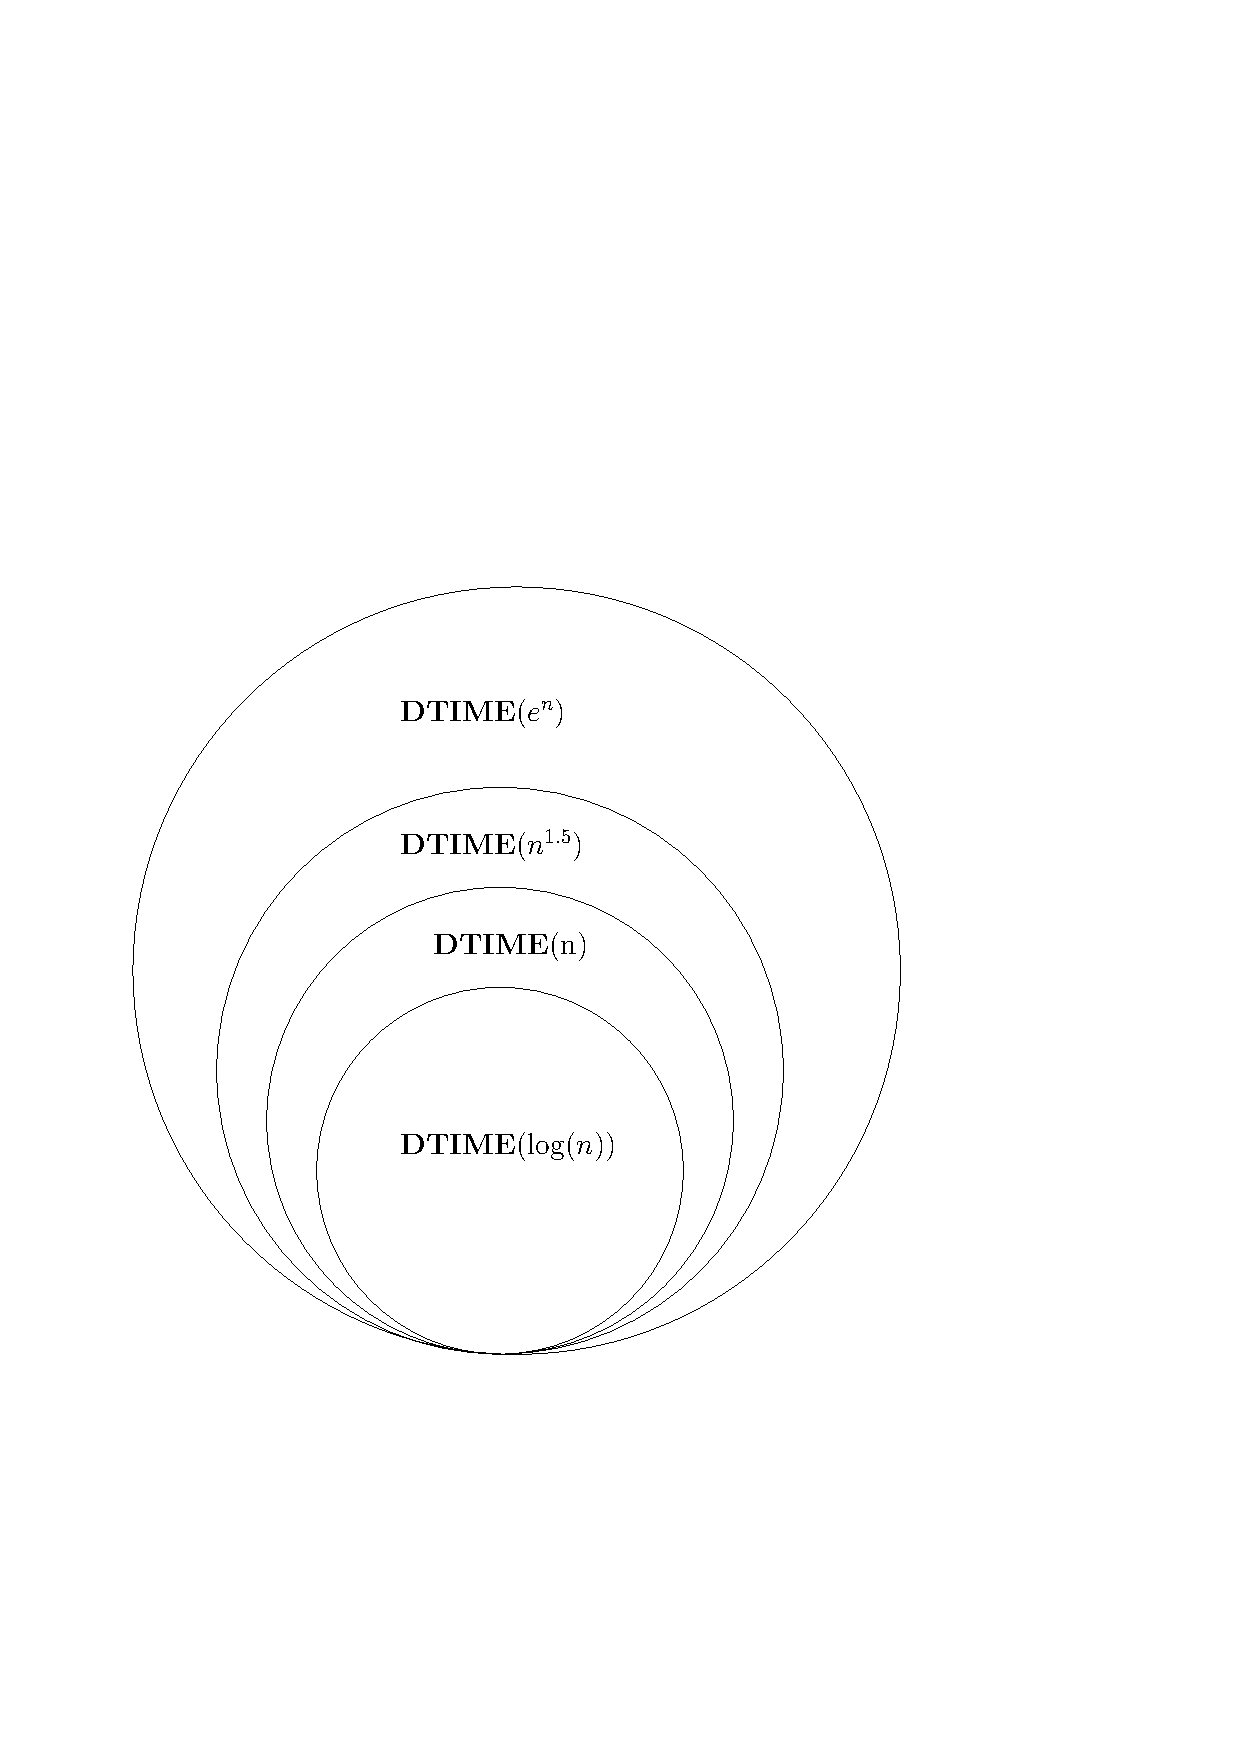
\includegraphics[scale=0.5]{timehierarchy.pdf}
\end{frame}
\subsection{Zweiter Unterabschnittstitel}

\begin{frame}{�berschriften m�ssen informativ sein.}
\end{frame}

\begin{frame}{�berschriften m�ssen informativ sein.}
\end{frame}

\section*{Zusammenfassung}

\begin{frame}{Zusammenfassung}

  % Die Zusammenfassung sollte sehr kurz sein.
  \begin{itemize}
  \item
    Die \alert{erste Hauptbotschaft} des Vortrags in ein bis zwei Zeilen.
  \item
    Die \alert{zweite Hauptbotschaft} des Vortrags in ein bis zwei Zeilen.
  \item
    Eventuell noch eine \alert{dritte Botschaft}, aber nicht noch mehr.
  \end{itemize}
  
  % Der folgende Ausblick ist optional.
  \vskip0pt plus.5fill
  \begin{itemize}
  \item
    Ausblick
    \begin{itemize}
    \item
      Etwas, was wir noch nicht l�sen konnten.
    \item
      Nochwas, das wir noch nicht l�sen konnten.
    \end{itemize}
  \end{itemize}
\end{frame}


\end{document}


